\documentclass[twocolumn]{article}
\usepackage{graphicx}

\title{
    \textbf{Programação 3D} \\
    Relatório Técnico da Primeira Entrega
}
\author{Afonso Mercier \and Pedro Quintas \and Pedro Caldeira}
\date{}

\begin{document}
    \maketitle

    \section{Funcionamento do Programa}

    O trabalho desenvolvido consiste numa aplicação de ray tracing na linguagem
    C++. O programa pode ser configurado para ler um ficheiro NFF e produz uma
    imagem fotorrealista com base na cena descrita no ficheiro. \\
    O desenvolvimento focou-se nos seguintes aspetos:

    \begin{itemize}
        \item Leitura de ficheiros NFF.
        \item Cálculo da componente local da cor.
        \item Suporte para multiplas fontes luminosas.
        \item Sombras de contorno rígido.
        \item Reflecção de raios.
        \item Refracção de raios.
        \item Intersecções de raios com algumas primitivas.
        \begin{itemize}
            \item Esferas
            \item Planos Infinitos
            \item Triângulos
            \item AABBs
        \end{itemize}
    \end{itemize}

    \section{Leitura de Ficheiros NFF}
    
    Ipsum Lorem

    \section{Componente Local da Cor}

    Ipsum Lorem

    \section{Fontes Luminosas}

    Ipsum Lorem

    \section{Sombras}

    Ipsum Lorem

    \section{Reflecção}

    Ipsum Lorem

    \section{Refracção}

    Ipsum Lorem

    \section{Intersecções}

    Ipsum Lorem

    \subsection{Esferas}

    Ipsum Lorem

    \subsection{Planos Infinitos}

    Ipsum Lorem

    \subsection{Triângulos}

    Ipsum Lorem

    \subsection{AABBs}

    Ipsum Lorem

    \newpage
    \null
    \newpage
    \section{Imagens}

    \begin{figure}[h!]
        \centering
        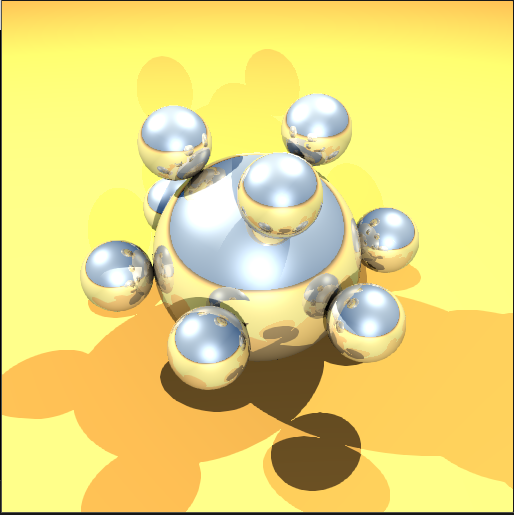
\includegraphics[width=200px]{balls_low.png}
        \caption{balls\_low.nff}
        \label{fig:balls_low}
    \end{figure}

    \begin{figure}[h!]
        \centering
        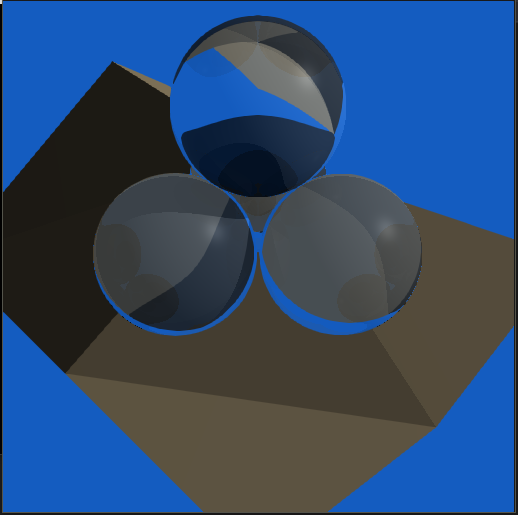
\includegraphics[width=200px]{mount_low.png}
        \caption{mount\_low.nff}
        \label{fig:mount_low}
    \end{figure}

    \begin{figure}[h!]
        \centering
        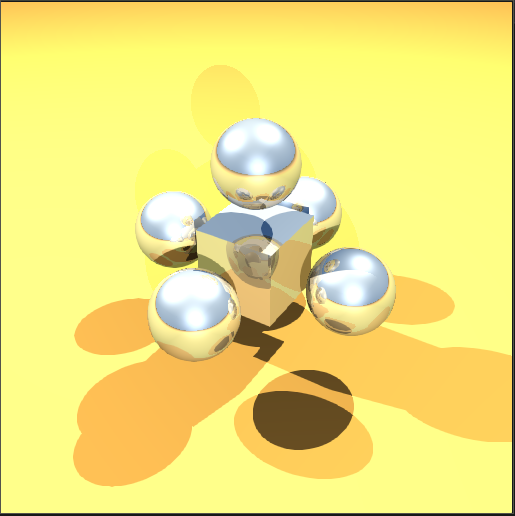
\includegraphics[width=200px]{aabb.png}
        \caption{aabb.nff}
        \label{fig:aabb}
    \end{figure}

\end{document}